\section{Introduktion}

\begin{frame}{\be-henfald}
	To typer:
	\begin{align*}
	\onslide<2->{&\beta^+:\quad p\rightarrow n + e^+ + \nu_e\\}
	\onslide<2->{&\beta^-:\quad n\rightarrow p + e^- + \bar{\nu_e}}
	\end{align*}
	\onslide<3->{Forskellige Q-værdier:}
	\begin{align*}
	\onslide<4->{&Q_{\beta^+} = \left[ m (\isotope[A][Z]{X}) - m(\isotope[A][Z-1]{X'})  		 \right] c^2\\
	&Q_{\beta^-} = \left[ m (\isotope[A][Z]{X}) - m(\isotope[A][Z+1]{X'}) -2m_e  \right] c^2}
	\end{align*}
\end{frame}

\begin{frame}{\be-henfald}
	Tilladte overgange:
	\begin{equation*}
	\onslide<2->{\Delta J = 0, \pm1,\ \Delta T = 0, \pm 1,\ \text{og}\ \Delta \pi = 0}
	\end{equation*}
	\onslide<3->{Spin, paritiet og isospin: $J^\pi ; T$}
	\onslide<4->{
		\begin{figure}
			\centering
			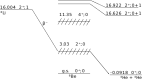
\includegraphics[width=.6\columnwidth]{../figures/DecayScheme.pdf}
		\end{figure}
	}
\end{frame}

\begin{frame}{\al-henfald}
	Udsendelsen af \al-partikel\\
	\onslide<2->{Q-værdi:
		\begin{equation*}
			Q_\alpha = \left[ m\left(^A_Z X\right) - m\left( ^{A-4}_{Z-2} X' \right) -m_\alpha \right]c^2
		\end{equation*}
	}
\end{frame}